\chapter{Математичне забезпечення методу автоматичної
ідентифікації музичних інструментів}

\label{chap:mathmodel}

Автоматична ідентифікація музичних інструментів у звуковому форматі
потребує вибору математичних методів на двох рівнях: методів цифрової
обробки сигналів для виділення тембрально релевантних ознак та методів
машинного навчання для multi-label класифікації. У даному розділі
розглянуто доступні математичні інструменти для кожного етапу обробки,
обґрунтовано вибір конкретних методів та наведено їх математичний опис.

% ------------------------------------------------------------------
\section{Постановка задачі multi-label класифікації}
\label{sec:problem_statement}

Задача автоматичної ідентифікації інструментів формалізується як задача
multi-label класифікації. Для кожного аудіофрагменту необхідно визначити
підмножину присутніх інструментів
\[
    \mathbf{y} \in \{0,1\}^K,
\]
де $K$ --- кількість класів інструментів, $y_k = 1$ означає присутність
$k$-го інструменту у записі.

На відміну від звичайної багатокласової класифікації, де рівно одна мітка
активна, у multi-label постановці кілька міток можуть бути активні
одночасно. Розв'язання задачі реалізує відображення
\[
    f_\theta : \mathbf{X} \rightarrow \hat{\mathbf{y}},
\]
де $\mathbf{X}$ --- матриця ознак аудіофрагменту, $\hat{\mathbf{y}} \in [0,1]^K$
--- вектор ймовірностей присутності кожного інструменту, $\theta$ ---
параметри моделі.

% ------------------------------------------------------------------
\section{Попередня обробка аудіосигналу}
\label{sec:preprocessing}

Нехай музичний твір задано у вигляді неперервного аудіосигналу
\[
    x(t), \quad t \in \mathbb{R}.
\]
Після дискретизації з частотою $f_s$ отримується дискретний сигнал
\[
    x[n] = x(n / f_s), \quad n = 1, 2, \dots, N.
\]

Аудіосигнал нормалізується за амплітудою та сегментується на перекривні
часові фрагменти довжини $L$ з кроком $H$:
\[
    x_t[n], \quad t = 1, 2, \dots, T.
\]
Такий підхід є загальноприйнятим у задачах аналізу музичних сигналів і
дозволяє отримати локальні часово-частотні представлення.

% ------------------------------------------------------------------
\section{Вибір методу часово-частотного аналізу}
\label{sec:timefreq}

Для переходу від часового до частотного представлення сигналу
застосовується перетворення Фур'є короткого вікна (STFT):
\[
    X_t(k) = \sum_{n=0}^{L-1} x_t[n]\, w[n]\, e^{-j 2 \pi k n / L},
\]
де $w[n]$ --- віконна функція. STFT формує комплексний спектр, модуль
якого використовується для подальшого обчислення енергетичного спектру.

На основі STFT будується мел-спектрограма, яка відображає спектральну
енергію у мел-шкалі частот. Мел-шкала є логарифмічною апроксимацією
частотного сприйняття людини і дозволяє компактно представити тембральні
характеристики інструментів.

% ------------------------------------------------------------------
\section{Мел-спектрограма та MFCC}
\label{sec:melspec}

Мел-спектрограма обчислюється шляхом застосування мел-фільтрбанку до
спектру STFT. Мел-фільтрбанк складається з $M$ трикутних фільтрів,
рівномірно розташованих у мел-шкалі:
\[
    S_t(m) = \sum_{k=0}^{L/2} |X_t(k)|^2 \cdot H_m(k),
    \quad m = 1, 2, \dots, M,
\]
де $H_m(k)$ --- частотна характеристика $m$-го фільтра.

Логарифм мел-спектрограми
\[
    \tilde{S}_t(m) = \log\!\left(S_t(m) + \epsilon\right)
\]
підкреслює структуру обертонів та формант, що є ключовою для
розрізнення тембрів інструментів.

Мел-частотні кепстральні коефіцієнти (MFCC) обчислюються шляхом
застосування дискретного косинусного перетворення (DCT) до
логарифмічної мел-спектрограми:
\[
    c_t(i) = \sum_{m=1}^{M} \tilde{S}_t(m)\, \cos\!\left(\frac{\pi i (m - 0.5)}{M}\right),
    \quad i = 1, 2, \dots, P.
\]

Мел-спектрограми та MFCC обрано як основне тембральне представлення
сигналу, оскільки вони є значно більш інформативними для задачі
ідентифікації тембру порівняно з хроматичними ознаками, що відображають
лише клас висоти звуку незалежно від тембру.

% ------------------------------------------------------------------
\section{Формування двовимірного подання для CNN}
\label{sec:cnn_input}

Мел-спектрограма природно представляється як двовимірна матриця
розмірності $M \times T$, де $M$ --- кількість мел-смуг, $T$ --- кількість
часових фреймів. Таке представлення інтерпретується як зображення:
\[
    \mathbf{S} \in \mathbb{R}^{M \times T},
\]
де рядки відповідають частотним смугам, а стовпці --- часовим фреймам.

Це дозволяє безпосередньо застосувати двовимірні згорткові фільтри для
виявлення локальних часово-частотних патернів, характерних для кожного
інструменту.

% ------------------------------------------------------------------
\section{Вибір архітектури моделі}
\label{sec:model_choice}

Для задачі multi-label класифікації інструментів розглянуто кілька класів
моделей, детально проаналізованих у розділі~\ref{chap:review}.

Класичні ML-методи (SVM, GMM) не враховують часовий контекст і
потребують ручного конструювання ознак. Виключно CNN-архітектури
дозволяють ефективно виявляти тембральні патерни у мел-спектрограмах,
проте не моделюють довгострокові часові залежності.

Гібридна архітектура CNN~+~BiLSTM поєднує переваги обох підходів:
\begin{itemize}
    \item CNN-блок витягує локальні тембральні ознаки зі
    спектрального представлення;
    \item BiLSTM-блок моделює часову динаміку звучання інструментів,
    враховуючи контекст у обох напрямках.
\end{itemize}

Таким чином, для multi-label класифікації обрано гібридну модель
CNN~+~BiLSTM як таку, що найповніше відповідає вимогам задачі.

\subsection{Математичний опис CNN-блоку}
\label{subsec:cnn_math}

CNN-блок складається з послідовності двовимірних згорткових шарів.
Операція згортки:
\[
    z^{(l)}(i,j) = \mathrm{ReLU}\!\left(\sum_{p,q} h^{(l)}(p,q)\, z^{(l-1)}(i+p, j+q) + b^{(l)}\right),
\]
де $h^{(l)}$ --- ядро фільтра $l$-го шару, $b^{(l)}$ --- зміщення.
Після операцій пулінгу вихід CNN-блоку має розмірність $C \times T'$,
де $C$ --- кількість карт ознак, $T'$ --- стиснений часовий вимір.

\subsection{Математичний опис BiLSTM-блоку}
\label{subsec:bilstm_math}

Послідовність карт ознак CNN-блоку подається на вхід BiLSTM. Прихований
стан формується шляхом об'єднання прямого та зворотного проходів:
\[
    \overrightarrow{\mathbf{h}}_t = g\!\left(\mathbf{x}_t,\,
    \overrightarrow{\mathbf{h}}_{t-1}\right), \quad
    \overleftarrow{\mathbf{h}}_t = g\!\left(\mathbf{x}_t,\,
    \overleftarrow{\mathbf{h}}_{t+1}\right),
\]
\[
    \mathbf{h}_t = \left[\overrightarrow{\mathbf{h}}_t;\,
    \overleftarrow{\mathbf{h}}_t\right],
\]
де $g(\cdot)$ --- нелінійна рекурентна функція LSTM-комірки.

% ------------------------------------------------------------------
\section{Вихідний шар та порогова функція}
\label{sec:output}

На відміну від задачі multiclass класифікації, де застосовується softmax,
у multi-label постановці для кожного класу використовується незалежна
сигмоїдна активація:
\[
    \hat{y}_k = \sigma(w_k^\top \mathbf{h} + b_k) = \frac{1}{1 + e^{-(w_k^\top \mathbf{h} + b_k)}},
    \quad k = 1, 2, \dots, K.
\]

Бінарне рішення про присутність $k$-го інструменту приймається за
порогом $\tau_k$:
\[
    \tilde{y}_k = \mathbb{1}[\hat{y}_k \geq \tau_k].
\]
Поріг $\tau_k = 0.5$ використовується за замовчуванням; при необхідності
він підбирається окремо для кожного класу на валідаційній вибірці.

% ------------------------------------------------------------------
\section{Функція втрат}
\label{sec:loss}

Для навчання моделі використовується бінарна крос-ентропія як стандартна
функція втрат для задач multi-label класифікації:
\[
    \mathcal{L}(\theta) = -\frac{1}{K}\sum_{k=1}^{K}
    \left[y_k \log \hat{y}_k + (1 - y_k) \log(1 - \hat{y}_k)\right].
\]
На відміну від категоріальної крос-ентропії, бінарна крос-ентропія
оцінює кожну мітку незалежно, що є природним для multi-label задачі.
Мінімізація функції втрат виконується методами стохастичної оптимізації.

% ------------------------------------------------------------------
\section{Концептуальна модель методу}
\label{sec:conceptual}

Концептуальна модель відображає логіку перетворення вхідного аудіосигналу
у вектор інструментальних міток та взаємозв'язки між обраними
математичними компонентами методу, як показано на
рисунку~\ref{fig:conceptual}.

Вхідний музичний аудіосигнал проходить попередню обробку, після чого
обчислюється мел-спектрограма. CNN-блок виявляє тембральні патерни у
спектральному поданні. BiLSTM-блок моделює часову динаміку. Вихідний
шар із сигмоїдною активацією та незалежними нейронами для кожного
класу формує вектор ймовірностей присутності інструментів.

\begin{figure}[H]
    \centering
    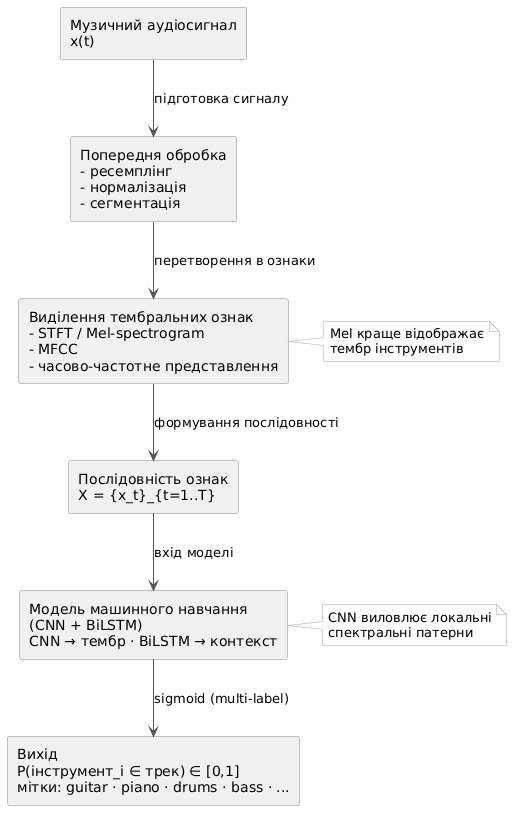
\includegraphics[width=0.7\textwidth]{Images/conceptual_model.png}
    \caption{Схема взаємодії компонентів методу}
    \label{fig:conceptual}
\end{figure}

% ------------------------------------------------------------------
\section{Висновки до розділу}
\label{sec:ch3_conclusions}

У розділі розглянуто математичні методи, доступні для кожного етапу
автоматичної ідентифікації інструментів, та обґрунтовано їх вибір.
Для виділення тембральних ознак обрано мел-спектрограму завдяки
відповідності мел-шкали частот особливостям слухового сприйняття та
інформативності для задачі розрізнення тембрів. Для класифікації
обрано гібридну архітектуру CNN~+~BiLSTM, яка поєднує виявлення
локальних тембральних патернів зі моделюванням часового контексту.
Задачу сформульовано як multi-label класифікацію з незалежними
сигмоїдними активаціями та бінарною крос-ентропійною функцією втрат.
